\chapter{Tris simples}

\begin{center}

\includegraphics[scale=0.4]{2_tri_selectif.png}   
\end{center}

\medskip

\begin{abstract}
    Dans ce chapitre nous allons donner deux algorithmes de tris de listes qui consistent à avancer pas-à-pas dans l'objectif souhaité. On en donnera l'analyse complète.
\end{abstract}
%-------------------------------------------------------------------------------
%-------------------------------------------------------------------------------
%-------------------------------------------------------------------------------
\section{Position du problème}
%-------------------------------------------------------------------------------
%-------------------------------------------------------------------------------
%-------------------------------------------------------------------------------
On a souvent besoin d'utiliser un ensemble trié d'éléments

\begin{itemize}
  \item pour déterminer le rang d'un élément,
  \item pour calculer la médiane,
  \item pour utiliser la recherche rapide d'un élément,
  \item pour sélectionner selon un critère,
  \item pour maintenir une liste de priorités,
  \item pour déterminer les résultats aberrants,
  \item \dots
\end{itemize}

\medskip

En pratique on se donne une collection d'éléments, en python ce sera une liste et on veut obtenir une liste triée.

On commence par préciser les termes ci-dessus.
%-------------------------------------------------------------------------------
%-------------------------------------------------------------------------------
\subsection{Relation d'ordre}
%-------------------------------------------------------------------------------
%-------------------------------------------------------------------------------
L'ordre provient de comparaisons entre éléments : leur ensemble est muni d'une relation d'ordre total. 

\begin{itemize}
  \item Ce peut être des nombres ou des chaînes de caractères, dans ce cas la relation d'ordre est définie dans Python par les relations \type{<, <=, >, >=}.
  \item Dans des cas plus généraux on devra définir une fonction à résultat booléen : par exemple \type{plusGrand(a,b)} qui devra renvoyer \type{True} si \type{a} est strictement supérieur à \type{b} pour la relation de comparaison et \type{False} si \type{a} est inférieur ou égal à \type{b}.
  
  On est dans ce cas, par exemple, dans le cas de listes ou de tuples dont une des composantes est un nombre, la clé. Les clés servent à la comparaison.
\end{itemize}

\medskip

{\bf La complexité sera calculée en comptant le nombre de comparaisons.}
%-------------------------------------------------------------------------------
\subsubsection{Exemple}
%-------------------------------------------------------------------------------
 Dans le tableau ci-dessous on veut trier en fonction de la note du DS4.
%-------------------------------------------------------------------------------
\begin{center}
\begin{tabular}{l|cccc}
nom       & DS1 & DS2 & DS3 & DS4 \\
\hline
André     & 10 & 12 & 15 &  9 \\ 
Bernard   &  8 & 16 &  7 & 14 \\ 
Céline    & 13 & 12 & 12 & 10 \\ 
Dominique &  8 &  6 &  9 &  8 \\ 
Éric      &  9 &  8 & 17 & 10 \\ 
François  & 14 & 13 & 12 & 15 \\ 
\end{tabular}
\end{center}
%-------------------------------------------------------------------------------
Les lignes sont représentées par des liste : \type{["André", 10, 12, 15, 9]}. 

La relation d'ordre est définie par la fonction
%-------------------------------------------------------------------------------
\begin{lstlisting}
def plusGrand(a,b):
    """Entrée : 2 éléments à comparer
       Sortie : True ssi a > b"""
    return a[4] > b[4]
\end{lstlisting}
%-------------------------------------------------------------------------------
On obtient 
%-------------------------------------------------------------------------------
\begin{center}
\begin{tabular}{l|cccc}
nom       & DS1 & DS2 & DS3 & DS4 \\
\hline
Dominique &  8 &  6 &  9 &  8 \\ 
André     & 10 & 12 & 15 &  9 \\ 
Céline    & 13 & 12 & 12 & 10 \\ 
Éric      &  9 &  8 & 17 & 10 \\ 
Bernard   &  8 & 16 &  7 & 14 \\ 
François  & 14 & 13 & 12 & 15 \\ 
\end{tabular}
\end{center}
%-------------------------------------------------------------------------------
Dans la suite, pour simplifier, nous illustrerons les tris avec des listes de nombres en employant les comparateurs internes de Python. 
%-------------------------------------------------------------------------------
%-------------------------------------------------------------------------------
\subsection{Résultat attendu}
%-------------------------------------------------------------------------------
%-------------------------------------------------------------------------------
On veut une liste triée, en général par ordre croissant : l'élément d'indice $i$ devra être plus inférieur ou égal à l'élément d'indice $i+1$.
\subsubsection{Tri externe ou en place}
%-------------------------------------------------------------------------------
Le résultat souhaité par un tri, "{\it on veut une liste triée}", est flou.

\begin{enumerate}
\item On peut souhaiter construire une nouvelle liste, triée, on parle alors de tri {\bf externe}.

L'avantage est qu'alors la liste initiale n'est pas détruite.

\item On peut souhaiter modifier la liste initiale, on trie {\bf en place}.

L'avantage est qu'on ne crée par une seconde liste ce qui peut être indispensable lorsque la liste à trier est très grande.
\end{enumerate}

La plupart des tris que nous étudierons seront des tris en place.

Les fonctions de tris seront alors des fonctions sans instruction \type{return}.

\medskip

Le docstring des tris sera donc, le plus souvent,
%-------------------------------------------------------------------------------
\begin{lstlisting}
def tri(liste):
    """Entrée : une liste d'éléments comparables
       Sortie : les éléments sont permutés pour obtenir
                une liste triée par ordre croissant"""
    ...
\end{lstlisting}
%-------------------------------------------------------------------------------
Dans le cas des tris en place, un outil souvent utilisé est une fonction de permutation qui échange deux éléments dans une liste. Une écriture de base est 
%-------------------------------------------------------------------------------
\begin{lstlisting}
def echange(liste,i,j):
    """Entree : une liste et deux indices i, j 
       Requis : 0 <= i,j < len(liste)
       Sortie : les termes i et j sont échangés"""
    temp = liste[i] # on sauvegarde liste[i]
    liste[i] = liste[j]
    liste[j] = temp
\end{lstlisting}
%-------------------------------------------------------------------------------

\subsubsection{Cas d'égalité}
%-------------------------------------------------------------------------------
Le résultat d'un tri est défini sans ambiguïté lorsque qu'il n'existe pas deux éléments distincts de la liste qui sont égaux pour la relation d'ordre

En cas d'égalité, comme dans l'exemple ci-dessus pour les lignes Céline et Éric,  il n'y a pas unicité de l'ordre final car on pourrait intervertir les deux lignes. 

On peut imposer que, comme dans l'exemple, les éléments indiscernables pour la relation d'ordre se retrouvent dans le même ordre à la fin.
%-------------------------------------------------------------------------------
\begin{defin}[Tri stable]
Un tri est stable si des éléments égaux pour la comparaison sont dans le même ordre dans le résultat final qu'à l'origine.
\end{defin}
%-------------------------------------------------------------------------------
%-------------------------------------------------------------------------------
%-------------------------------------------------------------------------------
\section{Tri par sélection}
%-------------------------------------------------------------------------------
%-------------------------------------------------------------------------------
%-------------------------------------------------------------------------------
Dans le tri par insertion on créait la liste triée en prenant un par un, comme ils venaient, les élément non encore triés. À chaque étape on doit alors modifier la partie triée.

On peut aussi construire directement la liste triée en mettant à leur place les éléments par ordre croissant. On sélectionne alors les élements : on parle de tri par sélection.
%-------------------------------------------------------------------------------
\begin{center}
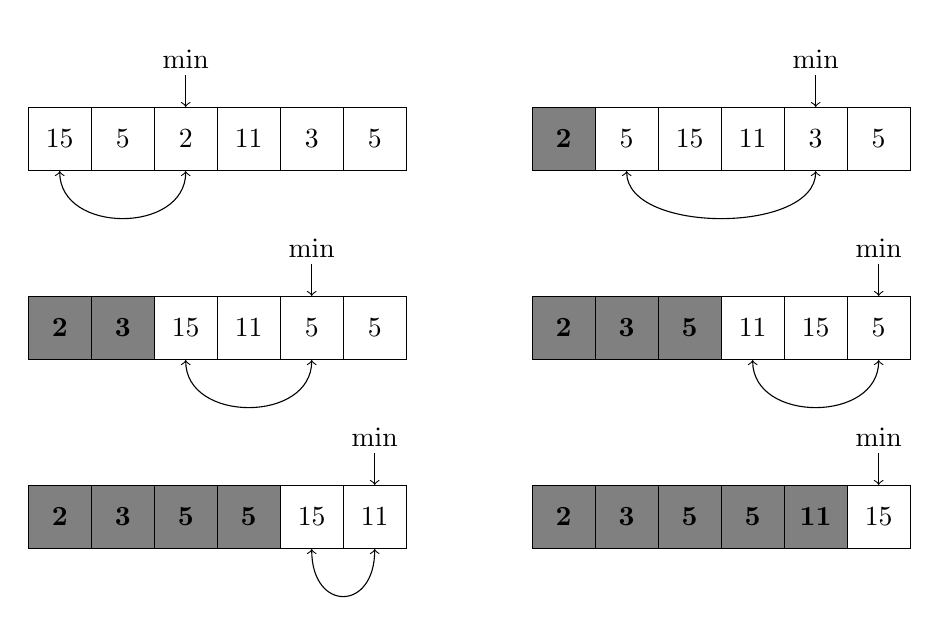
\begin{tikzpicture}[scale = 0.8,every node/.style={minimum size=0.8cm}]
  
\foreach \n/\v in {0/15,1/5,2/2,3/11,4/3,5/5}
\node[draw] (a\n) at (\n,0) {\v};
\draw [<-] (a2.north) -- +(0,0.5) node[above=-2mm]{min};
\draw[<->] (a0.south) ..controls +(0,-1) and +(0,-1) .. (a2.south);

\foreach \n/\v in {1/5,2/15,3/11,4/3,5/5}
\node[draw] (a\n) at (\n+8,0) {\v};
\draw [<-] (a4.north) -- +(0,0.5) node[above=-2mm]{min};
\draw[<->] (a1.south) ..controls +(0,-1) and +(0,-1) .. (a4.south);
\foreach \n/\v in {0/2}
\node[draw,fill=gray] (a\n) at (\n+8,0) {\bf \v};

\foreach \n/\v in {2/15,3/11,4/5,5/5}
\node[draw] (a\n) at (\n,-3) {\v};
\draw [<-] (a4.north) -- +(0,0.5) node[above=-2mm]{min};
\draw[<->] (a2.south) ..controls +(0,-1) and +(0,-1) .. (a4.south);
\foreach \n/\v in {0/2,1/3}
\node[draw,fill=gray] (a\n) at (\n,-3) {\bf \v};

\foreach \n/\v in {3/11,4/15,5/5}
\node[draw] (a\n) at (\n+8,-3) {\v};
\draw [<-] (a5.north) -- +(0,0.5) node[above=-2mm]{min};
\draw[<->] (a3.south) ..controls +(0,-1) and +(0,-1) .. (a5.south);
\foreach \n/\v in {0/2,1/3,2/5}
\node[draw,fill=gray] (a\n) at (\n+8,-3) {\bf \v};

  
\foreach \n/\v in {4/15,5/11}
\node[draw] (a\n) at (\n,-6) {\v};
\draw [<-] (a5.north) -- +(0,0.5) node[above=-2mm]{min};
\draw[<->] (a4.south) ..controls +(0,-1) and +(0,-1) .. (a5.south);
\foreach \n/\v in {0/2,1/3,2/5,3/5}
\node[draw,fill=gray] (a\n) at (\n,-6) {\bf \v};

\foreach \n/\v in {5/15}
\node[draw] (a\n) at (\n+8,-6) {\v};
\draw [<-] (a5.north) -- +(0,0.5) node[above=-2mm]{min};
\foreach \n/\v in {0/2,1/3,2/5,3/5,4/11}
\node[draw,fill=gray] (a\n) at (\n+8,-6) {\bf \v};

\end{tikzpicture}
\end{center}
%-------------------------------------------------------------------------------
À chaque étape on a déterminé le minimum parmi les termes restants et on l'a placé.

On a donc besoin d'une fonction qui recherche l'indice du minimum à partir d'un rang.

C'est un algorithme classique.
%-------------------------------------------------------------------------------
\begin{lstlisting}
def indMinDepuis(liste, i):
    """Entrées : une liste d'éléments compares par plusGrand
                 une entier i < len(liste)
       Sortie  : le premier indice en lequel la liste extraite
                 entre i et la fin atteint son minimum"""
    n = len(liste)
    ind_min = i
    mini = liste[i]
    for j in range(i+1,n):
        if plusGrand(mini, liste[j]):
            mini = liste[j]
            ind_min = j
    return ind_min 
\end{lstlisting}
%-------------------------------------------------------------------------------
On choisit la première apparition du minimum pour que le tri soit stable.

\medskip

On peut alors écrire la fonction de tri.
\begin{lstlisting}
def triSelection(liste):
    """Entrée : une liste d'éléments comparables par plusGrand
       Sortie : les éléments sont permutés pour obtenir
                une liste triée par ordre croissant"""
    n = len(liste)
    for i in range(n):
        k = indMinDepuis(liste, i)
        echange(liste, i, k)
\end{lstlisting}
On pourrait arrêter la boucle à $i=n-2$ car le dernier élément est à sa place quand on a placé les $n-1$ éléments les plus petits au début de la liste.
%-------------------------------------------------------------------------------
%-------------------------------------------------------------------------------
\subsection{Analyse}
%-------------------------------------------------------------------------------
%-------------------------------------------------------------------------------
\subsubsection{Terminaison}
Les fonctions n'utilisent que des boucles \type{for}, on est donc assurer qu'elles terminent.

\subsubsection{Preuve} On a construit la liste triée pas-à-pas.
%-------------------------------------------------------------------------------
\begin{lstlisting}
def triSelection(liste):
    n = len(liste)
    for i in range(n):
        # Les i premiers éléments de la liste triée
        # sont à leur place
        k = indMinDepuis(liste, i)
        echange(liste, i, k)
        # Les (i+1) premiers éléments de la liste triée
        # sont à leur place
\end{lstlisting}
%-------------------------------------------------------------------------------
À la fin de la boucle, $i$ a pris la valeur $n-1$ et la propriété implique que les $n-1+1$ premiers éléments de la liste triée sont à leur place : la liste est triée.

On doit donc s'assurer qu'on place le $i+1$-ième élément trié à la position $i$. Comme les $i$ premiers éléments, les plus petits, sont déjà placés, on doit choisir le minimum de ceux qui restent.

On peut prouver que \type{indMinDepuis(liste, i)} détermine bien le minimum en prouvant que \type{mini} contient, au début de la boucle pour $j$, le minimum des valeurs de la liste entre $i$ et $j-1$, c'est notrre invariant.

\medskip
Si on note $a_k$ la valeur de \type{liste[k]} et $m_{i, k} = \min\{a_i, a_{i+1}, \ldots, a_k\}$, l'algorithme calcule $m_j$ en fonction de $m_{j-1}$ en utilisant la propriété

$m_{j} = m_{j-1}$ si $a_j \ge m_{j-1}$ et $m_j= a_j$ sinon.

\subsubsection{Complexité} On effectue une comparaison pour chaque $j$ de $i+1$ à $n-1$ donc le nombre de comparaisons est $n-1-i$

On en déduit que le nombre de comparaisons de \type{triSelection} pour une liste de taille $n$  est donc
$\displaystyle C(n)=\sum_{i=0}^{n-1} (n-i-1)=\sum_{p=0}^{n-1} p = \frac{n(n-1)}2$, la complexité est un ${\cal O}\bigl(n^2\bigr)$. 

%-------------------------------------------------------------------------------
%-------------------------------------------------------------------------------
%-------------------------------------------------------------------------------
\section{Tri par insertion}
%-------------------------------------------------------------------------------
%-------------------------------------------------------------------------------
%-------------------------------------------------------------------------------
\subsection{Principe du tri}
%-------------------------------------------------------------------------------
%-------------------------------------------------------------------------------
Le tri par sélection est celui que les joueurs de cartes peuvent employer : pour trier un tas de carte, on prend une carte à la fois et on l'insère dans les cartes déjà triées.

Dans le cadre du tri en place d'une liste, on trie les éléments les uns après les autres en laissant en place ceux qu'on n'a pas encore considérés.

L'algorithme peut s'énoncer sous la forme
%-------------------------------------------------------------------------------
\begin{itemize}
\item Pour i allant de 0 à $n-1$ ($n$ est la longueur de la liste)
\item insérer le $i$-ième terme parmi les $i-1$ premiers en conservant le caractère trié.
\end{itemize}
%-------------------------------------------------------------------------------
On peut remarquer qu'on a, avant d'écrire le programme, un invariant de boucle :

pour chaque entier $i$ on a
%-------------------------------------------------------------------------------
\begin{itemize}
\item les $i$ premiers éléments de la liste (d'indices 0 à $i-1$) sont les $i$ premiers éléments de la liste initiale placés dans l'ordre
\item les derniers éléments (d'indices $i$ à $n-1$) sont les éléments d'origine de la liste, à leur place.
\end{itemize}
%-------------------------------------------------------------------------------

\medskip
On va représenter le principe le l'algorithme en montrant les étapes du tri à partir de la liste \type{[6, 9, 3, 8, 7, 2]}. Les listes ci-dessous sont représentées verticalement avec l'indice 0 en haut.
%-------------------------------------------------------------------------------
\begin{center}
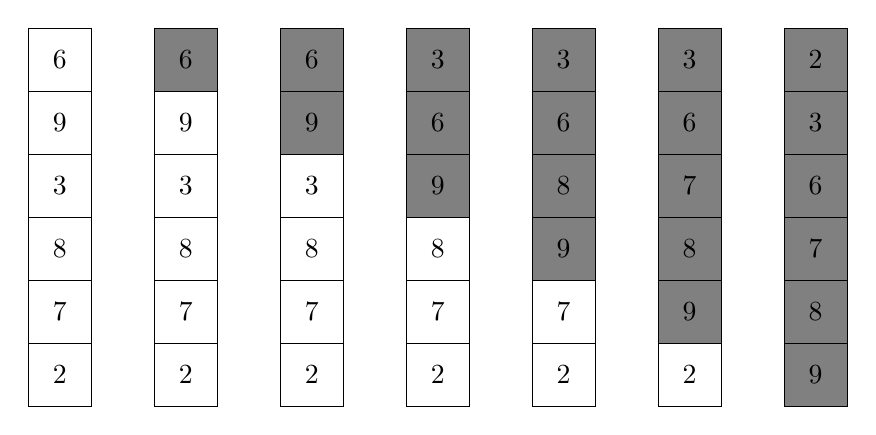
\begin{tikzpicture}[scale = 0.8,every node/.style={minimum size=0.8cm}]
\node[draw          ] (l_5) at (-2,0) {2};
\node[draw          ] (l_4) at (-2,1) {7};
\node[draw          ] (l_3) at (-2,2) {8};
\node[draw          ] (l_2) at (-2,3) {3};
\node[draw          ] (l_1) at (-2,4) {9};
\node[draw          ] (l_0) at (-2,5) {6};

\node[draw          ] (l05) at (0,0) {2};
\node[draw          ] (l04) at (0,1) {7};
\node[draw          ] (l03) at (0,2) {8};
\node[draw          ] (l02) at (0,3) {3};
\node[draw          ] (l01) at (0,4) {9};
\node[draw,fill=gray] (l00) at (0,5) {6};

\node[draw          ] (l15) at (2,0) {2};
\node[draw          ] (l14) at (2,1) {7};
\node[draw          ] (l13) at (2,2) {8};
\node[draw          ] (l12) at (2,3) {3};
\node[draw,fill=gray] (l11) at (2,4) {9};
\node[draw,fill=gray] (l10) at (2,5) {6};

\node[draw          ] (l25) at (4,0) {2};
\node[draw          ] (l24) at (4,1) {7};
\node[draw          ] (l23) at (4,2) {8};
\node[draw,fill=gray] (l22) at (4,3) {9};
\node[draw,fill=gray] (l21) at (4,4) {6};
\node[draw,fill=gray] (l20) at (4,5) {3};

\node[draw          ] (l35) at (6,0) {2};
\node[draw          ] (l34) at (6,1) {7};
\node[draw,fill=gray] (l33) at (6,2) {9};
\node[draw,fill=gray] (l32) at (6,3) {8};
\node[draw,fill=gray] (l31) at (6,4) {6};
\node[draw,fill=gray] (l30) at (6,5) {3};

\node[draw          ] (l45) at (8,0) {2};
\node[draw,fill=gray] (l44) at (8,1) {9};
\node[draw,fill=gray] (l43) at (8,2) {8};
\node[draw,fill=gray] (l42) at (8,3) {7};
\node[draw,fill=gray] (l41) at (8,4) {6};
\node[draw,fill=gray] (l40) at (8,5) {3};

\node[draw,fill=gray] (l55) at (10,0) {9};
\node[draw,fill=gray] (l54) at (10,1) {8};
\node[draw,fill=gray] (l53) at (10,2) {7};
\node[draw,fill=gray] (l52) at (10,3) {6};
\node[draw,fill=gray] (l51) at (10,4) {3};
\node[draw,fill=gray] (l50) at (10,5) {2};
\end{tikzpicture}
\end{center}
%-------------------------------------------------------------------------------
On peut donc écrire le programme suivant
%-------------------------------------------------------------------------------
\begin{lstlisting}
def triInsertion(liste):
    """Entrée : une liste d'éléments comparables 
       Sortie : les éléments sont permutés pour obtenir
                une liste triée par ordre croissant"""
    n = len(liste)
    for i in range(n):
        inserer(liste, i)
\end{lstlisting}
%-------------------------------------------------------------------------------
\newpage
%-------------------------------------------------------------------------------
%-------------------------------------------------------------------------------
\subsection{Insertion}
%-------------------------------------------------------------------------------
%-------------------------------------------------------------------------------
Pour réaliser \type{inserer(liste, i)} on peut itérer le procédé suivant en commençant par $k=i$.
%-------------------------------------------------------------------------------
\begin{enumerate}
\item Si $k=0$ on a fini.
\item Si on a $k> 0$ et si \type{liste[k-1] > liste[k]} on échange les éléments des positions $k$ et $k-1$ puis on diminue $k$ de 1 (on décrémente $k$).
\item Si on a $k> 0$ et si \type{liste[k-1] <= liste[k]} on a fini.
\end{enumerate}
%-------------------------------------------------------------------------------

Le fait de ne pas échanger en cas d'égalité donnera un tri stable.

{\bf Exemple} : exécution de \type{inserer(liste, 6)} 

avec \type{liste = [2, 7, 11, 13, 15, 18, 11, 24, 15, 5]}.
%-------------------------------------------------------------------------------
\begin{center}
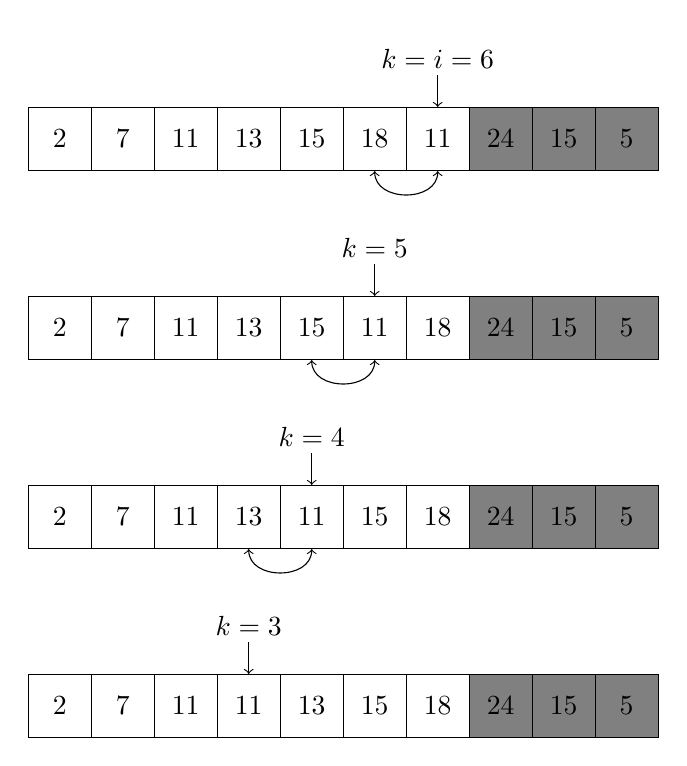
\begin{tikzpicture}[scale = 0.8,every node/.style={minimum size=0.8cm}]
\foreach \h in{0,-3,-6,-9}
 {\foreach \n/\v in {7/24,8/15,9/5}
  \node[draw,fill=gray] at (\n,\h) {\v};
  \foreach \n/\v in {0/2,1/7,2/11}
  \node[draw] at (\n,\h) {\v};
  };
  
\foreach \n/\v in {3/13,4/15,5/18,6/11}
\node[draw] (a\n) at (\n,0) {\v};
\draw [<-] (a6.north) -- +(0,0.5) node[above=-2mm]{$k=i=6$};
\draw[<->] (a6.south) ..controls +(0,-0.5) and +(0,-0.5) .. (a5.south);

\foreach \n/\v in {3/13,4/15,5/11,6/18}
\node[draw] (b\n) at (\n,-3) {\v};
\draw [<-] (b5.north) -- +(0,0.5) node[above=-2mm]{$k=5$};
\draw[<->] (b5.south) ..controls +(0,-0.5) and +(0,-0.5) .. (b4.south);

\foreach \n/\v in {3/13,4/11,5/15,6/18}
\node[draw] (c\n) at (\n,-6) {\v};
\draw [<-] (c4.north) -- +(0,0.5) node[above=-2mm]{$k=4$};
\draw[<->] (c4.south) ..controls +(0,-0.5) and +(0,-0.5) .. (c3.south);

\foreach \n/\v in {3/11,4/13,5/15,6/18}
\node[draw] (d\n) at (\n,-9) {\v};
\draw [<-] (d3.north) -- +(0,0.5) node[above=-2mm]{$k=3$};
\end{tikzpicture}
\end{center}
%-------------------------------------------------------------------------------
En appliquant ces idées on peut écrire le programme
%-------------------------------------------------------------------------------
%-------------------------------------------------------------------------------
\begin{lstlisting}
def inserer(liste, i):
    """Entrées : une liste d'éléments compares par plusGrand
                 une entier i < len(liste)
       Requis  : la liste est triée de 0 a i-1
       Sortie  : la liste est triée entre 0 et i"""
    k = i
    while k > 0:
        if plusGrand(liste[k-1], liste[k]):
            echange(liste, k, k-1)
            k = k - 1
        else:
            break
\end{lstlisting}
%-------------------------------------------------------------------------------
%-------------------------------------------------------------------------------
\subsection{Analyse}
%-------------------------------------------------------------------------------
%-------------------------------------------------------------------------------
\subsubsection{Terminaison} La fonction \type{inserer} termine car l'entier \type{k} décroît strictement à chaque passage de la boucle donc finit par être nul si n'est pas sorti de la boucle auparavant.

La fonction \type{triInsertion} fait appel $n-1$ fois à la fonction  \type{inserer} qui termine donc le tri termine.

\subsubsection{Preuve} On veut que la liste soit triée : pour cela on trie des portions de plus en plus grandes.

On introduit une propriété vérifiée lors du passage de la boucle.
%-------------------------------------------------------------------------------
\begin{lstlisting}
def triInsertion(liste):
    n = len(liste)
    for i in range(n):
        # Les i premiers éléments de la liste sont triés, 
        # les autres sont inchangés
        inserer(liste, i)
        # Les i+1 premiers éléments de la liste sont triés, 
        # les autres sont inchangés
   # Les n éléments de la liste sont triés
\end{lstlisting}
%-------------------------------------------------------------------------------
À la fin de la boucle, $i$ a pris la valeur $n-1$ et la propriété implique que les $n-1+1$ premiers éléments sont triés : la liste est triée.

On doit donc prouver que \type{inserer(liste, i)} transforme la propriété de $i$ à $i+1$.

On note $a_j$ la valeur de \type{liste[j]}.
%-------------------------------------------------------------------------------
\begin{center}
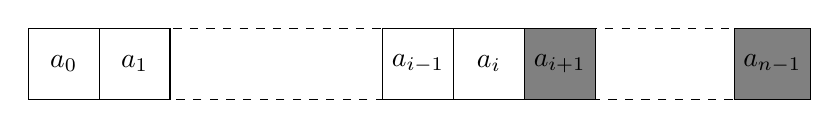
\begin{tikzpicture}[scale = 0.9,every node/.style={minimum size=0.9cm}]
\draw[dashed](-0.5, -0.5) rectangle (10.5, 0.5);
\node[draw] at (0, 0) {$a_0$};
\node[draw] at (1, 0) {$a_1$};
\node[draw] at (5, 0) {$a_{i-1}$};
\node[draw] at (6, 0) {$a_i$};
\node[draw,fill=gray] at (7, 0) {$a_{i+1}$};
\node[draw,fill=gray] at (10, 0) {$a_{n-1}$};
\end{tikzpicture}
\end{center}
%-------------------------------------------------------------------------------
 On peut remarquer que les transformations successives donnent des résultats
%-------------------------------------------------------------------------------
\begin{center}
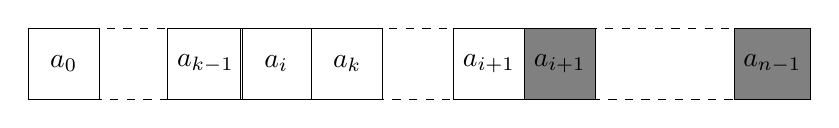
\begin{tikzpicture}[scale = 0.9,every node/.style={minimum size=0.9cm}]
\draw[dashed](-0.5, -0.5) rectangle (10.5, 0.5);
\node[draw] at (0, 0) {$a_0$};
\node[draw] at (2, 0) {$a_{k-1}$};
\node[draw] at (3, 0) {$a_i$};
\node[draw] at (4, 0) {$a_{k}$};
\node[draw] at (6, 0) {$a_{i+1}$};
\node[draw,fill=gray] at (7, 0) {$a_{i+1}$};
\node[draw,fill=gray] at (10, 0) {$a_{n-1}$};
\end{tikzpicture}
\end{center}
%-------------------------------------------------------------------------------
On peut exprimer ces positions par les propriétés
%-------------------------------------------------------------------------------
\begin{lstlisting}
liste[0] <= liste[1]   <= ... <= liste[k-1]
liste[k] <= liste[k+1] <= ... <= liste[n-1]
liste[k-1] <= liste[k]
\end{lstlisting}
%-------------------------------------------------------------------------------
On prouve alors que les instructions 
%-------------------------------------------------------------------------------
\begin{lstlisting}
echange(liste, k, k-1)
            k = k - 1
\end{lstlisting}
%-------------------------------------------------------------------------------
conservent les propriétés, elles forment un invariant, lorsque l'on a \type{liste[k] < liste [k-1]}.

Par contre, si on a \type{liste[k] >= liste [k-1]},  la portion de 0 à $i$ est triée donc on a le résultat souhaité.

De même, pour $k=0$ la portion est triée aussi.

Ainsi la fonction \type{inserer} produit bien le résultat souhaité.

\subsubsection{Complexité} On effectue une comparaison pour chaque $k$ de $i$ à $k_0$ avec $1\le k_0 \le i$ donc le nombre de comparaisons est compris entre 1 et $i$ pour \type{inserer(liste, i)}.

On en déduit que le nombre de comparaisons de \type{triInsertion} pour une liste de taille $n$, $C(n)$ vérifie 
$\displaystyle \sum_{i=0}^{n-1} 1 = n  \le C(n) \le   \sum_{i=0}^{n-1} i = \frac{n(n-1)}2$, la complexité est un ${\cal O}\bigl(n^2\bigr)$. 

D'après l'étude de la fonction  \type{inserer} la complexité maximale est atteinte lorsque l'élément d'indice $i$ est inférieur (strictement) à tous ceux qui le précèdent, pour chaque $i$ : c'est le cas pour une liste strictement décroissante au départ.

De même la complexité est minimale pour une liste strictement croissante au départ.

Le tri par insertion est préférable au tri par sélection, il peut être très rapide dans le cas de liste qui sont peu désordonnées. On l'emploie parfois dans des tris plus rapides lors des dernières étapes pour lesquelles la liste est triée par blocs.

Si on compte aussi les échanges, on voit que le tri par sélection ne fait que $n$ échanges alors que le tri par insertion en effectue en 0 et $\frac{n(n-1)}2$.
%-------------------------------------------------------------------------------
\newpage
%-------------------------------------------------------------------------------
\subsection{Un exemple de complexité moyenne}
%-------------------------------------------------------------------------------
%-------------------------------------------------------------------------------
On rappelle qu'on compte le nombre de comparaisons pour déterminer la complexité.

Comme la complexité du tri par insertion est variable, on peut souhaiter calculer sa {\bf complexité moyenne} pour les listes de taille $n$. On ne peut pas calculer la moyenne sur toutes les listes de taille $n$ car il y en a une infinité.
On considère plus simplement comme toutes les permutations d'une liste de $n$ éléments {\bf distincts}, il y en a $n!$.

Pour une liste $L = [a_1, a_2, \ldots, a_{n}]$ d'éléments distincts, on note $L_\sigma$ la liste obtenue en permutant les termes avec la permutation $\sigma$ : $L_\sigma = [a_{\sigma(1)}, \ldots, a_{\sigma(n)}]$. 

La complexité moyenne recherchée est donc $\displaystyle \overline C(n) = \frac 1{n!}\sum_{\sigma\in S_n} C(L_\sigma)$
où $C(L_\sigma)$ est le nombre de comparaisons effectuées lors du tri par insertion de $L_\sigma$.

On remarque que cette moyenne ne dépend pas de la liste $L$ avec $n$ termes distincts.

On a vu que $\displaystyle C(L_\sigma) = \sum_{i=0}^{n-1} C_{ins}(L_\sigma, i)$ où $C_{ins}(L_\sigma, i)$ est le nombre de comparaisons effectuées lors de l'insertion du terme d'indice $i$ parmi les $i$ premieres.

Si le terme d'indice $i$ est placé à la position $j$, on a comparé le terme avec $L_{\sigma}[i-1]$, $L_{\sigma}[i-2]$ jusqu'à $L_{\sigma}[j-1]$ pour $j\ge 0$, soit $i-j+1$ comparaisons. Si le terme d'indice $i$ est placé à la position $0$ on ne fait que $i$ comparaisons. Si on note $C_{ins}(L_\sigma, i, j)$ le nombre de comparaisons effectuées pour insérer le terme d'indice $i$ en $j$, on a donc $C_{ins}(L_\sigma, i, j) = i-j+1$ pour $1\le j\le j$ et $C_{ins}(L_\sigma, i, 0) = i$
 
On admet que les emplacements possible pour le terme d'indice $i$ lors de son insertion sont équiprobables. Il y a $i+1$ valeurs possibles, de 0 à $i$, chacune obtenue par $\frac{n!}{i+1}$ permutations. Ainsi

\begin{align*}
\frac 1{n!}\sum_{\sigma\in S_n} C_{ins}(L_\sigma, i)
&=\frac 1{n!} \sum_{j=0}^{i} \frac{n!}{i+1}C_{ins}(L_\sigma, i, j)
=\frac{1}{i+1}\left(i + \sum_{j=1}^i (i-j+1)\right)\\
&=\frac{1}{i+1}\left(i + + \sum_{k=1}^i k\right)
=\frac{1}{i+1}\left(i + \frac{i(i+1)}2\right)\\
&=\frac{i}{2}+\frac{i}{i+1}
=\frac{i}{2}+1 - \frac 1{i+1}
\end{align*}

On conclut donc
\begin{align*}
\overline C(n) 
&= \frac 1{n!}\sum_{\sigma\in S_n} C(L_\sigma)
=\frac 1{n!}\sum_{\sigma\in S_n} \left(\sum_{i=0}^{n-1} C_{ins}(L_\sigma, i)\right)
= \sum_{i=0}^{n-1}\left(\frac 1{n!}\sum_{\sigma\in S_n} C_{ins}(L_\sigma, i)\right)\\
&=\sum_{i=0}^{n-1}\left(\frac{i}{2}+1 - \frac 1{i+1}\right)
=\frac{n(n-1)}4 + n -\sum_{p=1}^n \frac 1p
=\frac {n^2} 4 + \frac{3n}4 - \sum_{p=1}^n \frac 1p
\end{align*}

La complexité moyenne reste quadratique, il y a simplement une division par 2 du terme en $n^2$.

% %-------------------------------------------------------------------------------
% %-------------------------------------------------------------------------------
% \begin{Exercise}[title={Simplification de l'insertion}]
% Dans la fonction \type{placer} du tri par insertion on fait 3 affectations lors de chaque échange.

% Un des éléments qui intervient dans l'échange est toujours le même.

% Proposer une fonction qui demande moins d'affectations.
% \end{Exercise}
% %------------------------------------------------------------
% \begin{Answer}
% Il suffit de copier les grands éléments à leur droite et, à la fin, de placer l'élément à insérer à sa place. Il ne faut pas oublier de mettre cet élément dans une variable.

% \begin{lstlisting}
% def inserer(liste,i):
%     """Entrées : une liste d'éléments comparables par plusGrand
%                  une entier i < len(liste)
%       Requis  : la liste est triée de 0 a i-1
%       Sortie  : la liste est triée entre 0 et i"""
%     cle = liste[i]
%     k = i
%     while k > 0 and plusGrand(liste[k-1],cle):
%         liste[k] = liste[k-1]
%         k = k - 1
%     liste[k] = cle
% \end{lstlisting}
% On fait $p+1$ affectations au lieu de $3p$ si la boucle est effectuée $p$ fois.
% \end{Answer}
% %------------------------------------------------------------
% %------------------------------------------------------------


% \begin{Exercise}[title={Complexité moyenne du tri par insertion}]
% On commence par évaluer la complexité moyenne en nombre de comparaisons de 

% \type{inserer(liste, i)} avec $i\ge 1$ : $\overline C_{ins}(i)$. On fait les hypothèses :
% \begin{enumerate}
% \item la liste est triée entre les indices 0 et $i-1$,
% \item (*) les positions de \type{liste[i]} après l'insertion sont équiprobables.
% \end{enumerate}
% En comptant le nombre de comparaisons pour chaque position prouver que le nombre moyen de comparaisons est $\displaystyle \overline C_{ins}(i) = \frac i2 + 1-\frac 1{i+1}$.

% \medskip

% Pour calculer la complexité moyenne du tri par insertion en nombre de comparaisons on considère toutes les permutations d'une liste de $n$ éléments {\bf distincts} et on admet qu'alors l'hypothèse (*) est vérifiée pour chaque $i$. 
% Prouver que le nombre moyen de comparaisons pour le tri par insertion des listes de taille $n$ est
% $\displaystyle \overline C(n) = \frac{n^2+3n}4-\sum_{k=1}^n \frac 1k$.
% \end{Exercise}
% %------------------------------------------------------------
% \begin{Answer}
% On note $k_0$ la position où aboutit \type{liste[i]}.

% Pour arriver à $k$ on doit échanger \type{liste[k]} et \type{liste[k-1]} pour $k\in\{i,i-1,\ldots,k_0+1\}$ : à chaque fois on a fait une comparaison. Si $k_0$ est non nul on doit faire une dernière comparaison pour finir la boucle.
% On fait $i+1-k_0$ comparaisons pour $k>0$ et $i$ comparaisons pour $k_0=0$. Chaque position à une probabilité de $\frac 1{i+1}$ donc

% $\displaystyle \overline C_{ins}(i) =
% \frac 1{i+1}\left(i + \sum_{k_0=1}^i i+1-k_0\right)=
% \frac 1{i+1}\left(i + \sum_{p=1}^i p\right)=
% \frac {i+\frac{i(i+1)}2}{i+1}=
% \frac i2 +\frac i{i+1}$

% \medskip

% Il suffit alors de sommer les moyennes

% \begin{align*}
% \overline C(n) 
% &
% = \sum_{i=1}^{n-1} \frac i2 + 1-\frac 1{i+1}
% =\frac 12 \sum_{i=1}^{n-1} i + n-1-\sum_{i=1}^{n-1} \frac 1{i+1}
% =\frac 12\frac{n(n-1)}2 + n-1-\sum_{p=2}^n \frac 1p 
% \\ &
% =\frac{n(n-1)}4 + n-\sum_{p=1}^n \frac 1p
% =\frac {n^2} 4 + \frac{3n}4 - \sum_{p=1}^n \frac 1p
% \end{align*}

% La complexité moyenne est donc de l'ordre de la moitié de la complexité maximale.
% \end{Answer}
% %-------------------------------------------------------------------------------
% %-------------------------------------------------------------------------------
% \subsection{Autres tris}
% %-------------------------------------------------------------------------------
% %-------------------------------------------------------------------------------
% \begin{Exercise}[title={Tri à bulles, CCP 2015}]
% On considère la fonction
% \begin{lstlisting}
% from copy import copy
% def trier(p):
%     t = copy(p)
%     for i in range(len(t)):         # boucle externe
%         for j in range(len(t)-i-1): # boucle interne
%             if (t[j+1]<t[j]):
%                 t[j], t[j+1] = t[j+1], t[j]
%     return t
% \end{lstlisting}
% \begin{enumerate}
% \item Montrer que la fonction termine.
% \item Combien de comparaison sont effectuées dans le cas d'une liste de taille $n$ ?
% \item Prouver que la fonction renvoie une liste avec les mêmes éléments que la liste initiale en les plaçant dans l'ordre croissant. On pourra, en plus de la conservation de l'ensemble des valeurs, utiliser les invariants de boucles suivants.

% $P_1(i)$ pour la boucle externe : 

% $\forall k \in\{n-i-1,\ldots,n-2\}$, \type{t[k] <= t[k+1]} et \type{t[k] <= t[n-i]}.

% $P_2(i,j)$ pour la boucle interne : $P_1(i)$ et $\forall k \in\{0,1,\ldots,j\}$, \type{t[k] <= t[j]}.
% \end{enumerate}
% \end{Exercise}
% %------------------------------------------------------------
% \begin{Answer}
% \begin{enumerate}
% \item Il n'y a que des itérations par des boucles \type{for} donc la fonction termine.
% \item Il y a 1 comparaison pour chaque passage donc le nombre est

% $\displaystyle \sum_{i=0}^{n-1} \sum_{j=0}^{n-2-i}1
% =  \sum_{i=0}^{n-1} n-1-i
% =  \sum_{k=0}^{n-1} k = \frac {n(n-1)}2$

% \item $P_1(0)$ n'a pas d'objet car on a $n-1> n-2$ et \type{t[n]} n'existe pas, elle est donc valide.

% Si $P_1(i)$ est valide pour $i < n-1$ on rentre dans la boucle interne avec $j=0$.
% \begin{itemize}
% \item $P_2(i,0)$ demande simplement \type{t[0] <= t[0]}.
% \item Si $P_2(i,j)$ est vérifiée avec $j<n-i-2$ et \type{t[j+1] < t[j]} alors on échange les termes d'indices $j$ et $j+1$. On note \type{t'} la nouvelle liste obtenue. On a \type{t'[j] = t[j+1] < t[j] = t'[j+1]} et \type{t'[k] = t[k] <= t[j] = t'[j+1]} pour $k< j$. Comme $P_1(i)$ reste vraie on a $P_2(i,j+1)$ est valide.
% \item Si \type{t[j+1] >= t[j]} alors la liste est inchangée.  On a \type{t[j] <= t[j+1]} et \type{t[k] <= t[j] <= t[j+1]} pour $k< j$ donc $P_2(i,j+1)$ est valide.
% \item $P_2(i,n-i-1)$ signifie qu'on a, à la position $n-i-1$, un majorant des éléments précédents qui est majoré par \type{t[n-i]} : cela implique, avec $P_1(i)$ la propriété $P_1(i+1)$.
% \end{itemize}

% $P_1(n-1)$ prouve alors que la liste est triée (il ne se passe rien pour $i=n-1$).
% \end{enumerate}
% \end{Answer}
% %------------------------------------------------------------
% %------------------------------------------------------------
% \begin{Exercise}[title={Un tri très rapide ?}]
% On suppose que l'on veut trier une liste d'éléments dont les clés sont des entiers {\bf distincts} et appartenant à un ensemble $\{0, 1, 2 ,\ldots, N-1\}$.

% Proposer une méthode de tri sans comparaison qui utilise une liste de taille $N$.

% La clé de tri est fournie par une fonction \type{cle}.

% Déterminer sa complexité : pourquoi ce tri n'est-il pas utilisé ?
% \end{Exercise}
% %------------------------------------------------------------
% \begin{Answer}
% On crée une liste de taille $N$ avec la valeur -1 (par exemple), on place l'élément $i$ à la place $i$ puis on lit les éléments distincts de -1 dans l'ordre. C'est tri qui renvoie une nouvelle liste.
% \begin{lstlisting}
% def tri(liste, N):
%     """Entrées : une liste d'entiers distincts
%                  compris entre 0 et N-1
%       Sortie  : la liste triée des éléments"""
%     casier= [-1]*N
%     n = len(liste)
%     for i in range(n):
%         k = cle(liste[i])
%         casier[k] = liste[i]
%     sortie = []
%     for i in range(N):
%         if casier[i] != -1:
%             sortie.append(casier[i])
%     return sortie
% \end{lstlisting}

% On ne fait aucune comparaison, on fait $n+N$ lectures et $2n$ écritures.

% Si $N$ n'est pas trop grand (majoré par $10n$ par exemple) on obtient un tri très rapide car linéaire. En général $N$ est trop grand pour qu'il soit raisonnable de créer une liste de taille $N$, c'est ce qui rend le tri peu utilisable.

% Un cas particulier et caricatural est celui où on veut trier une permutation des $n$ premier entiers : il suffit de renvoyer \type{list(range(n))} sans jamais lire la liste passée en paramètre.
% \end{Answer}
% %------------------------------------------------------------
% %------------------------------------------------------------
% \begin{Exercise}[title={Cas particulier}]
% L'idée de l'exercice précédent peut cependant être utilisée dans un cas particulier.

% On suppose que l'on veut trier une liste d'éléments dont les clés sont des entiers appartenant à un ensemble $\{0, 1, 2 ,\ldots, N-1\}$. L'entier $N$ est "petit" par rapport à la taille de la liste mais plusieurs élément peuvent avoir la même clé. C'est ce qui se produit, par exemple, quand on veut trier une liste d'étudiants en fonction de la note d'un devoir.

% Proposer une méthode de tri sans comparaison qui utilise une liste de listes, de taille $N$.
% \end{Exercise}
% %------------------------------------------------------------
% \begin{Answer}
% Une liste de liste vides ne peut pas être créée par \type{[]*N}.
% \begin{lstlisting}
% def tri(liste, N):
%     """Entrées : une liste d'entiers distincts
%                  compris entre 0 et N-1
%       Sortie  : la liste triée des éléments"""
%     casier= [[] for i in range(N)]
%     for item in liste:
%         k = cle(item)
%         casier[k].append(item)
%     sortie = []
%     for paquet in casier:
%         for item in paquet:
%             sortie.append(item)
%     return sortie
% \end{lstlisting}

% On fait $2n$ utilisations de \type{append} et $N+2n$ lectures.

% \newpage
% \end{Answer}
% %------------------------------------------------------------
% %------------------------------------------------------------
% \begin{Exercise}[title={Tri d'une liste de 4 éléments}]

% Pour trier une liste de 4 éléments le tri par insertion peut demander jusqu'à 

% $\frac{4(4-1)}2=6$ comparaisons (le tri par sélection en demande toujours 6).

% Donner une fonction qui trie en place une liste de longueur 4 en effectuant au plus 5 comparaisons (et au plus 5 appels de \type{echange}).
% \end{Exercise}
% %------------------------------------------------------------
% \begin{Answer}
% \begin{lstlisting}
% def tri4(liste):
%     """Entrée : une liste de 4 éléments
%       Sortie : la liste est triée"""
%     if plusGrand(liste[0],liste[2]):
%         echange(0,2,liste)
%     if plusGrand(liste[1],liste[3]):
%         echange(1,3,liste)
%     if plusGrand(liste[0],liste[1]):
%         echange(0,1,liste)
%     if plusGrand(liste[2],liste[3]):
%         echange(2,3,liste)
%     if plusGrand(liste[1],liste[2]):
%         echange(1,2,liste)
% \end{lstlisting}

% \newpage
% \end{Answer}
% %------------------------------------------------------------
% %------------------------------------------------------------
